\section{ĐỊNH LUẬT CHARLES}
\subsection{LÝ THUYẾT TRỌNG TÂM}
\begin{boxdl}
	Khi áp suất của một khối lượng khí xác định được giữ không đổi thì thể tích của khí tỉ lệ thuận với nhiệt độ tuyệt đối của nó:
	\begin{equation}
		\dfrac{V}{T}=\text{hằng số}\quad \text{hay} \quad \dfrac{V_1}{T_1}=\dfrac{V_2}{T_2}
	\end{equation}
\end{boxdl}
\begin{minipage}[t]{.45\linewidth}
	\begin{center}
		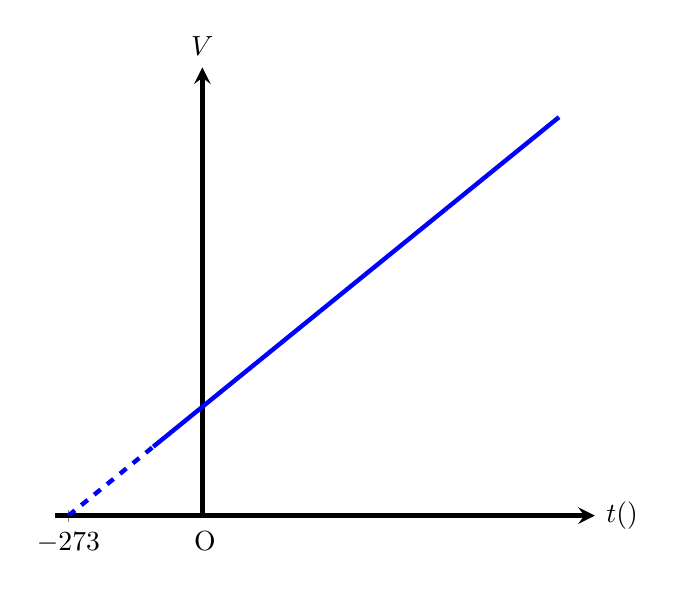
\begin{tikzpicture}  
			\begin{axis}[  ultra thick,
				xmin=-300,  
				xmax=800,  
				xtick={-273,0},
				ytick=\empty,
				ymin=0,  
				ymax=900, 
				samples=300,
				%				xticklabels=\empty,
				yticklabels=\empty,
				axis lines=center, 
				xlabel=$\xsi{t}{(\celsius)}$, 
				ylabel=$V$, 
				every axis y label/.style={at=(current axis.above origin),anchor=south},  
				every axis x label/.style={at=(current axis.right of origin),anchor=west},  ]
				\addplot [ultra thick, blue, smooth,dashed, domain=-273:-100] {0.8*(x+273)}; 
				\addplot [ultra thick, blue, smooth, domain=-100:727] {0.8*(x+273)}; 
			\end{axis}  
			\node[label={[below]90:O}] at (1.9,-0.2){};
		\end{tikzpicture}
		\captionof{figure}{Đồ thị biểu diễn sự thay đổi thể tích khí theo nhiệt độ Celsius}
	\end{center}
\end{minipage}\hfill
\begin{minipage}[t]{.45\linewidth}
	\begin{center}
		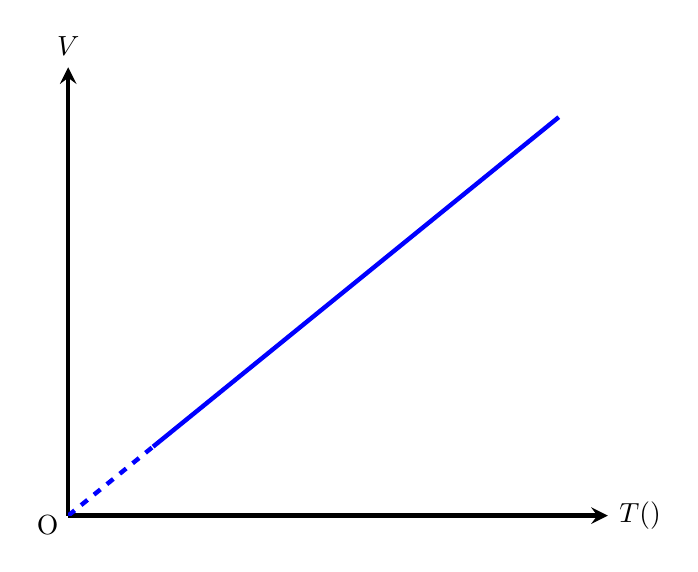
\begin{tikzpicture}  
			\begin{axis}[  ultra thick,
				xmin=0,  
				xmax=1100,  
				xtick=\empty,
				ytick=\empty,
				ymin=0,  
				ymax=900, 
				samples=300,
				xticklabels=\empty,
				yticklabels=\empty,
				axis lines=center, 
				xlabel=$\xsi{T}{(\kelvin)}$, 
				ylabel=$V$, 
				every axis y label/.style={at=(current axis.above origin),anchor=south},  
				every axis x label/.style={at=(current axis.right of origin),anchor=west},  ]
				\addplot [ultra thick, blue, smooth,dashed, domain=0:173] {0.8*x}; 
				\addplot [ultra thick, blue, smooth, domain=173:1000] {0.8*x}; 
			\end{axis}  
			\node[label={[below left]90:O}] at (0,0){};
		\end{tikzpicture}
		\captionof{figure}{Đồ thị biểu diễn sự thay đổi thể tích khí theo nhiệt độ Kelvin}
	\end{center}
\end{minipage}
\begin{center}
	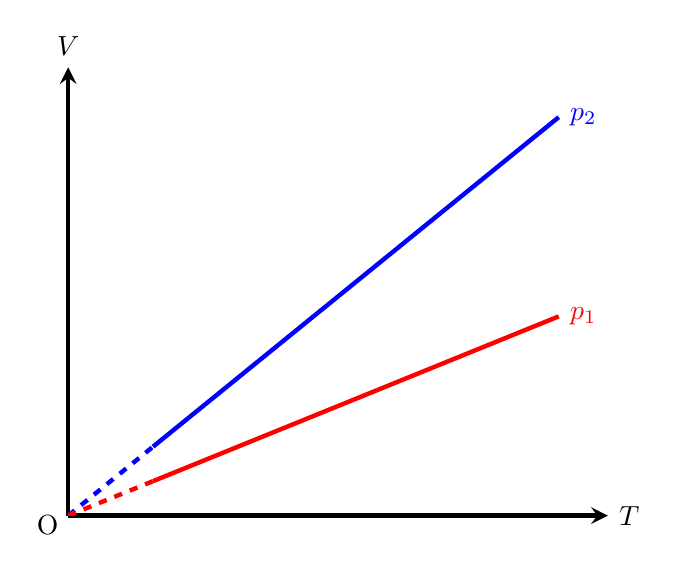
\begin{tikzpicture}  
		\begin{axis}[  ultra thick,
			xmin=0,  
			xmax=1100,  
			xtick=\empty,
			ytick=\empty,
			ymin=0,  
			ymax=900, 
			samples=300,
			xticklabels=\empty,
			yticklabels=\empty,
			axis lines=center, 
			xlabel=$T$, 
			ylabel=$V$, 
			every axis y label/.style={at=(current axis.above origin),anchor=south},  
			every axis x label/.style={at=(current axis.right of origin),anchor=west},  ]
			\addplot [ultra thick, blue, smooth,dashed, domain=0:173] {0.8*x}; 
			\addplot [ultra thick, blue, smooth, domain=173:1000] {0.8*x} node[right]{$p_2$}; 
			\addplot [ultra thick, red, smooth,dashed, domain=0:173] {0.4*x}; 
			\addplot [ultra thick, red, smooth, domain=173:1000] {0.4*x} node[right]{$p_1$};
		\end{axis}  
		\node[label={[below left]90:O}] at (0,0){};
	\end{tikzpicture}
	\captionof{figure}{Các đường đẳng áp của một khối khí lí tưởng ứng với các áp suất $p_1$ và $p_2 \left(p_2<p_1\right)$}
\end{center}
\begin{luuy}
	Định luật Boyle và định luật Charles là các định luật đúng với khí lí tưởng, gần đúng với khí thực. Trong điều kiện áp suất cao và nhiệt độ thấp, kết quả thực nghiệm khí thực không phù hợp với các định luật trên.
\end{luuy}
\subsection{VÍ DỤ MINH HOẠ}
\begin{dang}{Vận dụng được định luật Charles}
\end{dang}
\begin{vd}
	Cho một khối khí dãn nở đẳng áp từ nhiệt độ $t_1=\SI{32}{\celsius}$ đến nhiệt độ $t_2=\SI{117}{\celsius}$, thể tích khối khí tăng thêm 1,7 lít. Xác định thể tích khối khí trước và sau khi dãn nở.
	\loigiai{
			\begin{center}
				\begin{tabular}{C{4cm} C{1.5cm} C{4.5cm}}
					\colorbox{yellow}{\textcolor{red}{\textbf{Trạng thái 1}}} & $\xrightarrow[]{p=const}$ & \colorbox{yellow}{\textcolor{red}{\textbf{Trạng thái 2}}}\\
					$T_1=\SI{305}{\kelvin}$ & &$T_2=\SI{390}{\kelvin}$\\
					$V_1=?$ & & $V_2=V_1+\SI{1.7}{\text{lít}}$
				\end{tabular}
			\end{center}
			Theo định luật Charles:
			\begin{eqnarray*}
				&&\dfrac{V_1}{T_1}=\dfrac{V_2}{T_2}\\
				&\Leftrightarrow& \dfrac{V_1}{\SI{305}{\kelvin}}=\dfrac{V_1+\SI{1.7}{\text{lít}}}{\SI{390}{\kelvin}}\\
				&\Rightarrow& V_1=\SI{6.1}{\text{lít}}.
			\end{eqnarray*}
	}
\end{vd}
% =================================================================================
\begin{vd}
Một mô hình áp kế gồm một bình cầu thuỷ tinh có thể tích $\SI{270}{\centi\meter^3}$ gắn với một ống nhỏ nằm ngang có tiết diện $\SI{0.1}{\centi\meter^2}$. Trong ống có một giọt thuỷ ngân. Ở $\SI{0}{\celsius}$ giọt thuỷ ngân cách miệng bình cầu $\SI{30}{\centi\meter}$. Tính khoảng di chuyển của giọt thuỷ ngân khi hơ nóng bình cầu đến $\SI{10}{\celsius}$. Coi thể tích bình là không đổi và ống thuỷ tinh đủ dài để giọt thuỷ ngân không rơi ra ngoài.
		\begin{center}
			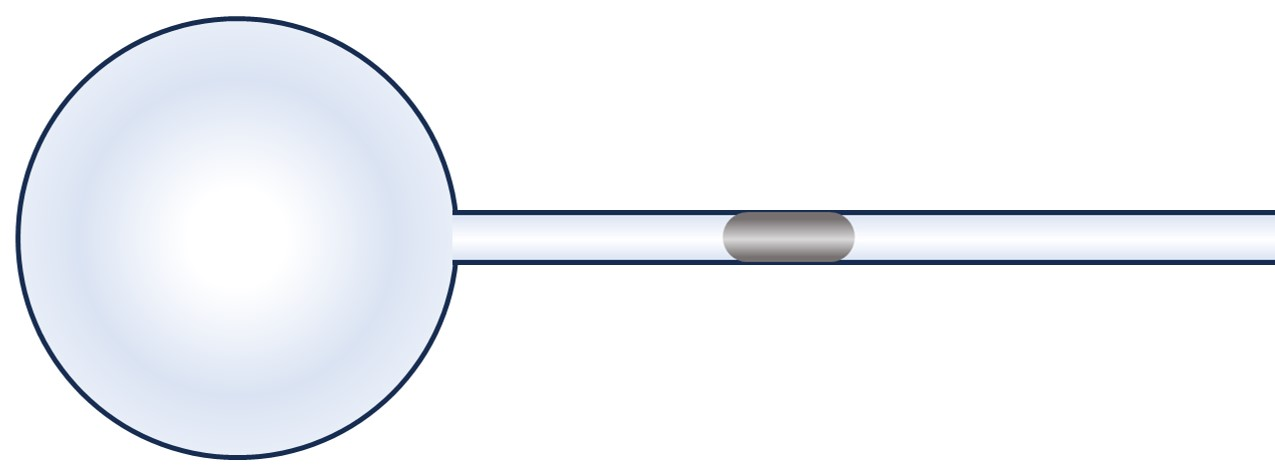
\includegraphics[width=0.35\linewidth]{figs/VN12-Y24-PH-SYL-011-1}
		\end{center}
\loigiai{
			Gọi:
			\begin{itemize}
				\item $S$ là tiết diện ống thuỷ tinh, $S=\SI{0.1}{\centi\meter^2}$;
				\item $V$ là thể tích bình cầu;
				\item $\ell_1$, $\ell_2$ lần lượt là khoảng cách từ giọt thuỷ ngân đến miệng bình trước và sau khi hơ nóng.
			\end{itemize} 
			Giọt thuỷ ngân cân bằng khi áp suất khí trong bình cân bằng với áp suất khí ngoài bình. Do đó, quá trình hơ nóng bình xem như quá trình biến đổi trạng thái đẳng áp của khí trong bình.
			\begin{center}
				\begin{tabular}{C{4cm} C{1.5cm} C{5cm}}
					\colorbox{yellow}{\textcolor{red}{\textbf{Trạng thái 1}}} & $\xrightarrow[]{p=const}$ & \colorbox{yellow}{\textcolor{red}{\textbf{Trạng thái 2}}}\\
					$T_1=\SI{273}{\kelvin}$ & &$T_2=\SI{283}{\kelvin}$\\
					$V_1=V+\ell_1S=\SI{273}{\centi\meter^3}$ & & $V_2=V+\ell_2S=\xsi{\left(270+0,1\ell_2\right)}{\centi\meter^3} $
				\end{tabular}
			\end{center}
			Theo định luật Charles:
			\begin{eqnarray*}
				&&\dfrac{V_1}{T_1}=\dfrac{V_2}{T_2}\\
				&\Leftrightarrow& \dfrac{\SI{273}{\centi\meter^3}}{\SI{273}{\kelvin}}=\dfrac{\xsi{\left(270+0,1\ell_2\right)}{\centi\meter^3}}{\SI{283}{\kelvin}}\\
				&\Rightarrow& \ell_2=\SI{130}{\centi\meter}
			\end{eqnarray*}
			Vậy: giọt thuỷ ngân đã di chuyển 1 đoạn $\Delta \ell=\ell_2-\ell_1=\SI{100}{\centi\meter}$.
	}
\end{vd}	
\subsection{BÀI TẬP TRẮC NGHIỆM}
\setcounter{ex}{0}
\Opensolutionfile{ans}[ans/G12Y24B10TN]
% ===================================================================
\begin{ex}
	Hệ thức nào sau đây \textbf{không phù hợp} với quá trình đẳng áp?
	\choice
	{$\dfrac{V}{T}=\text{const}$}
	{\True $V\sim\dfrac{1}{T}$}
	{$V\sim T$}
	{$\dfrac{V_1}{T_1}=\dfrac{V_2}{T_2}$}
	\loigiai{}
\end{ex}
% ===================================================================
\begin{ex}
	\immini{
Một thí nghiệm được thực hiện với khối không khí chứa trong bình cầu 
và ngăn với khí quyển bằng giọt thủy ngân như hình vẽ. Khi làm nóng hay nguội  bình cầu thì biến đổi của khối khí thuộc loại nào?
}{
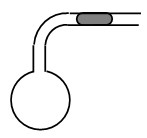
\includegraphics[scale=0.5]{figs/VN12-Y24-PH-SYL-011P-3}
}
	\choice
	{\True Đẳng áp}
	{Đẳng tích}
	{Đẳng nhiệt}
	{Bất kì}
	\loigiai{}
\end{ex}
% ===================================================================
\begin{ex}
	Trong hệ toạ độ $OVT$, đường biểu diễn nào sau đây là đường đẳng áp?
	\choice
	{Đường thẳng song song với trục hoành}
	{Đường thẳng song song với trục tung}
	{Đường hyperbol}
	{\True Đường thẳng kéo dài đi qua gốc toạ độ}
	\loigiai{}
\end{ex}
% ===================================================================
\begin{ex}
	Một quả bóng bay chứa khí hydrogen vào buổi sáng ở nhiệt độ $\SI{20}{\celsius}$ thì có thể tích $\SI{2500}{\centi\meter^3}$. Coi áp suất khí quyển trong ngày không đổi. Thể tích của quả bóng này vào buổi trưa có nhiệt độ $\SI{35}{\celsius}$ \textbf{gần nhất} với giá trị nào sau đây?
	\choice
	{$\SI{4375}{\centi\meter^3}$}
	{\True $\SI{2628}{\centi\meter^3}$}
	{$\SI{2378}{\centi\meter^3}$}
	{$\SI{1429}{\centi\meter^3}$}
	\loigiai{\begin{center}
			\begin{tabular}{C{4cm} C{3cm} C{4cm}}
				\colorbox{yellow}{\textcolor{red}{\textbf{Trạng thái 1}}} & $\xrightarrow[]{p_1=p_2}$ & \colorbox{yellow}{\textcolor{red}{\textbf{Trạng thái 2}}}\\
				$V_1=\SI{2500}{\centi\meter^3}$ & &$V_2=?$\\
				$T_1=\SI{293}{\kelvin}$ & & $T_2=\SI{308}{\kelvin}$
			\end{tabular}
			
		\end{center}
		$$\dfrac{V_1}{T_1}=\dfrac{V_2}{T_2}\Rightarrow V_2\approx\SI{2628}{\centi\meter^3}.$$
	}
\end{ex}
% ===================================================================
\begin{ex}
Ở nhiệt độ $\SI{273}{\celsius}$ thể tích của một khối khí lí tưởng là $\SI{10}{\liter}$. Trong điều kiện áp suất không đổi, thể tích của khối khí đó ở nhiệt độ $\SI{546}{\celsius}$ là	
	\choice
	{$\SI{20}{\liter}$}
	{\True $\SI{15}{\liter}$}
	{$\SI{12}{\liter}$}
	{$\SI{13.5}{\liter}$}
	\loigiai{\begin{center}
			\begin{tabular}{C{4cm} C{3cm} C{4cm}}
				\colorbox{yellow}{\textcolor{red}{\textbf{Trạng thái 1}}} & $\xrightarrow[]{p_1=p_2}$ & \colorbox{yellow}{\textcolor{red}{\textbf{Trạng thái 2}}}\\
				$V_1=\SI{10}{\liter}$ & &$V_2=?$\\
				$T_1=\SI{546}{\kelvin}$ & & $T_2=\SI{819}{\kelvin}$
			\end{tabular}
		\end{center}
		$$\dfrac{V_1}{T_1}=\dfrac{V_2}{T_2}\Rightarrow V_2=\SI{15}{\liter}.$$
	}
\end{ex}
% ===================================================================
\begin{ex}
	Một khối khí lí tưởng ban đầu có các thông số trạng thái $p_0$; $V_0$; $T_0$. Khối khí biến đổi đẳng áp đến thể tích $2V_0$ rồi biến đổi đẳng nhiệt về thể tích ban đầu. Đồ thị nào sau đây diễn tả \textbf{đúng} quá trình trên?
	\begin{center}
		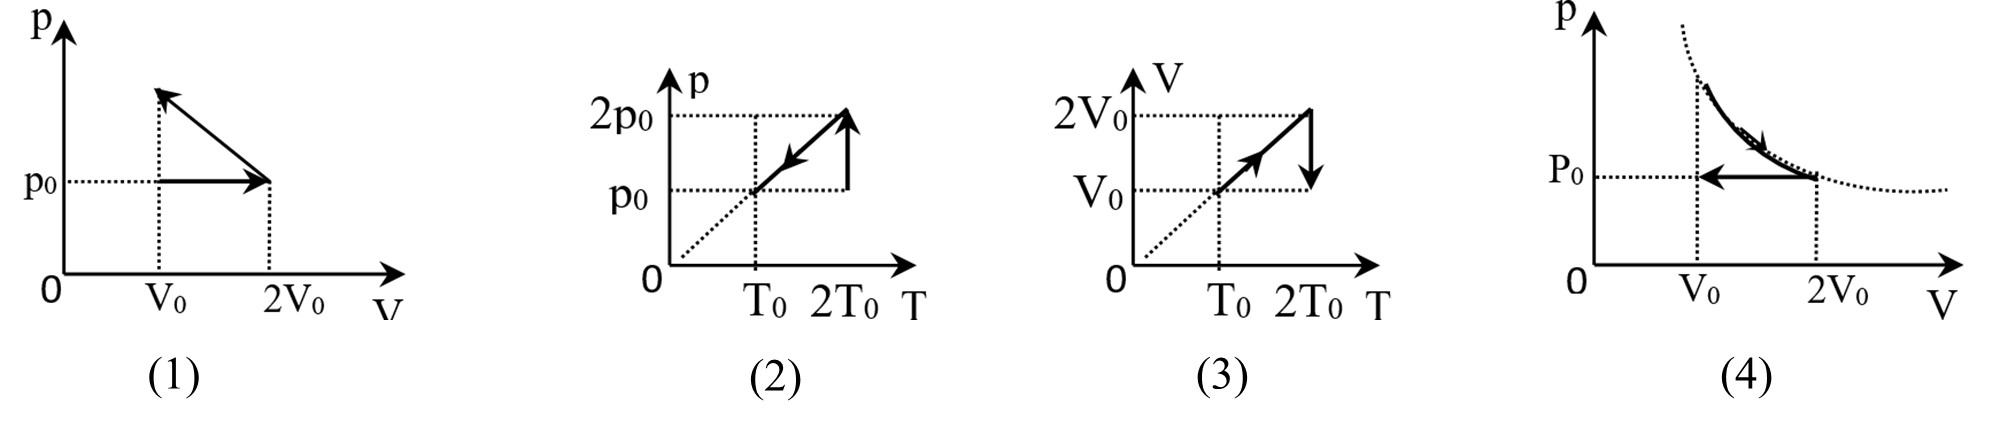
\includegraphics[width=0.9\linewidth]{figs/VN12-Y24-PH-SYL-011P-4}
	\end{center}
	\choice
	{(1)}
	{(2)}
	{\True (3)}
	{(4)}
	\loigiai{}
\end{ex}
% ===================================================================
\begin{ex}
	Thể tích của một lượng khí xác định tăng thêm $\SI{10}{\percent}$  khi nhiệt độ của khí được tăng tới $\SI{47}{\celsius}$. Xác định nhiệt độ ban đầu của lượng khí, biết quá trình trên là đẳng áp.
	
	\choice
	{\True $\SI{18}{\celsius}$}
	{$\SI{42}{\celsius}$}
	{$\SI{51.7}{\celsius}$}
	{$\SI{79}{\celsius}$}
	\loigiai{$$\dfrac{T_1}{T_2}=\dfrac{V_1}{V_2}\Rightarrow T_1=\dfrac{T_2}{1,1}\approx\SI{291}{\kelvin}\Rightarrow t_1=\SI{18}{\celsius}.$$
	}
\end{ex}
% ===================================================================
\begin{ex}
Một khối khí có thể tích $\SI{10}{\liter}$ ở $\SI{27}{\celsius}$. Giữ cho áp suất của khối khí không thay đổi, phải tăng nhiệt độ của khối khí lên bao nhiêu độ nữa để thể tích của nó là $\SI{12}{\liter}$?
	
	\choice
	{$\SI{300}{\kelvin}$}
	{$\SI{360}{\kelvin}$}
	{\True $\SI{60}{\kelvin}$}
	{$\SI{120}{\kelvin}$}
	\loigiai{\begin{center}
			\begin{tabular}{C{4cm} C{3cm} C{4cm}}
				\colorbox{yellow}{\textcolor{red}{\textbf{Trạng thái 1}}} & $\xrightarrow[]{p_1=p_2}$ & \colorbox{yellow}{\textcolor{red}{\textbf{Trạng thái 2}}}\\
				$V_1=\SI{10}{\liter}$ & &$V_2=\SI{12}{\liter}$\\
				$T_1=\SI{300}{\kelvin}$ & & $T_2=?$
			\end{tabular}
		\end{center}
		$$\dfrac{V_1}{T_1}=\dfrac{V_2}{T_2}\Rightarrow T_2=\SI{360}{\kelvin}\Rightarrow \Delta T=\SI{60}{\kelvin}.$$
	}
\end{ex}
% ===================================================================
\begin{ex}
Khi nhiệt độ của khối khí lí tưởng tăng từ $\SI{27}{\celsius}$ đến $\SI{227}{\celsius}$ đồng thời giữ khối lượng và áp suất khí không đổi thì thể tích của khí sẽ
	
	\choice
	{\True tăng lên $\SI{66.67}{\percent}$}
	{giảm xuống $\SI{66.67}{\percent}$}
	{tăng lên $\SI{40}{\percent}$}
	{giảm xuống $\SI{40}{\percent}$}
	\loigiai{$$\dfrac{V_2}{V_1}=\dfrac{T_2}{T_1}=\dfrac{5}{3}\approx\SI{166.67}{\percent}.$$
	}
\end{ex}
% ===================================================================
\begin{ex}
	Một khối khí $\SI{12}{\gram}$ có thể tích $\SI{4}{\liter}$ ở nhiệt độ $\SI{7}{\celsius}$. Sau khi được đun nóng đẳng áp thì khối lượng riêng của khí là $\SI{1.2}{\gram/\liter}$. Nhiệt độ của khí sau khi được đun nóng là
	
	\choice
	{$\SI{84}{\celsius}$}
	{$\SI{574}{\celsius}$}
	{$\SI{247}{\celsius}$}
	{\True $\SI{427}{\celsius}$}
	\loigiai{\begin{center}
			\begin{tabular}{C{4cm} C{3cm} C{4cm}}
				\colorbox{yellow}{\textcolor{red}{\textbf{Trạng thái 1}}} & $\xrightarrow[]{p_1=p_2}$ & \colorbox{yellow}{\textcolor{red}{\textbf{Trạng thái 2}}}\\
				$V_1=\SI{4}{\liter}$ & &$V_2=\SI{10}{\liter}$\\
				$T_1=\SI{280}{\kelvin}$ & & $T_2=?$
			\end{tabular}
		\end{center}
	}
\end{ex}
% ===================================================================
\begin{ex}
	Nung nóng một lượng khí trong điều kiện đẳng áp, người ta thấy  khi nhiệt độ của khối khí tăng thêm $\SI{3}{\kelvin}$ thì thể tích tăng thêm $\SI{1}{\percent}$ so với thể tích ban đầu. Nhiệt độ ban đầu của lượng khí trên là
	
	\choice
	{$\SI{17}{\celsius}$}
	{$\SI{56}{\celsius}$}
	{\True $\SI{27}{\celsius}$}
	{$\SI{36}{\celsius}$}
	\loigiai{\begin{center}
			\begin{tabular}{C{4cm} C{3cm} C{4cm}}
				\colorbox{yellow}{\textcolor{red}{\textbf{Trạng thái 1}}} & $\xrightarrow[]{p_1=p_2}$ & \colorbox{yellow}{\textcolor{red}{\textbf{Trạng thái 2}}}\\
				$V_1$ & &$V_2=1,01V_1$\\
				$T_1=?$ & & $T_2=T_1+3$
			\end{tabular}
		\end{center}
		Theo định luật Charles:
		$$\dfrac{T_1}{V_1}=\dfrac{T_1+3}{1,01V_1}\Rightarrow T_1=\SI{300}{\kelvin}\Rightarrow t_1=\SI{27}{\celsius}.$$
	}
\end{ex}
% ===================================================================
\begin{ex}
	Ống thuỷ tinh tiết diện đều với một đầu kín và một đầu hở. Bên trong ống có cột không khí dài $\ell_1=\SI{20}{\centi\meter}$ được ngăn cách với không khí bên ngoài bởi cột thuỷ ngân, nhiệt độ bên trong ống là $\SI{27}{\celsius}$. Khi nhiệt độ không khí bên trong ống tăng thêm $\SI{10}{\celsius}$ thì chiều cao cột không khí bên trong ống là bao nhiêu nếu áp suất của khí không đổi?
	
	\choice
	{$\SI{22}{\centi\meter}$}
	{$\SI{19.68}{\centi\meter}$}
	{\True $\SI{20.67}{\centi\meter}$}
	{$\SI{18.96}{\centi\meter}$}
	\loigiai{\begin{center}
			\begin{tabular}{C{4cm} C{3cm} C{4cm}}
				\colorbox{yellow}{\textcolor{red}{\textbf{Trạng thái 1}}} & $\xrightarrow[]{p_1=p_2}$ & \colorbox{yellow}{\textcolor{red}{\textbf{Trạng thái 2}}}\\
				$V_1=\ell_1S$ & &$V_2=\ell_2S$\\
				$T_1=\SI{300}{\kelvin}$ & & $T_2=\SI{310}{\kelvin}$
			\end{tabular}
		\end{center}
		$$\dfrac{V_1}{T_1}=\dfrac{V_2}{T_2}\Rightarrow \ell_2\approx\SI{20.67}{\centi\meter}.$$
	}
\end{ex}
% ===================================================================
\begin{ex}
	Một bình dung tích $V=\SI{15}{\centi\meter^3}$ chứa không khí ở nhiệt độ $t_1=\SI{177}{\celsius}$ nối với một ống nằm ngang chứa đầy thuỷ ngân, đầu kia của ống thông với không khí bên ngoài. Khối lượng riêng của thuỷ ngân là $\SI{13.6}{\gram/\centi\meter^3}$. Khi nhiệt độ trong bình được làm lạnh đến nhiệt độ $t_2=\SI{27}{\celsius}$ thì khối lượng thuỷ ngân chảy vào bình là
	
	\choice
	{$\SI{5}{\gram}$}
	{$\SI{172.88}{\gram}$}
	{\True $\SI{68}{\gram}$}
	{$\SI{136}{\gram}$}
	\loigiai{\begin{center}
			\begin{tabular}{C{4cm} C{3cm} C{4cm}}
				\colorbox{yellow}{\textcolor{red}{\textbf{Trạng thái 1}}} & $\xrightarrow[]{p_1=p_2}$ & \colorbox{yellow}{\textcolor{red}{\textbf{Trạng thái 2}}}\\
				$V_1=\SI{15}{\centi\meter^3}$ & &$V_2=?$\\
				$T_1=\SI{450}{\kelvin}$ & & $T_2=\SI{300}{\kelvin}$
			\end{tabular}
		\end{center}
		$$\dfrac{V_1}{T_1}=\dfrac{V_2}{T_2}\Rightarrow V_2=\SI{10}{\centi\meter^3}.$$
		Thể tích thuỷ ngân chảy vào bình là
		$$\Delta V=V_2-V_1=\SI{5}{\centi\meter^3}.$$
		Khối lượng thuỷ ngân chảy và bình là
		$$\Delta m=\rho \Delta V=\SI{68}{\gram}.$$}
\end{ex}
% ===================================================================
\begin{ex}
	Cho áp kế như hình vẽ. Ống thuỷ tinh dài có tiết diện $\SI{0.1}{\centi\meter^2}$. Ở $\SI{0}{\celsius}$ giọt thuỷ ngân cách A là $\SI{30}{\centi\meter}$, ở $\SI{5}{\celsius}$ giọt thuỷ ngân cách A là $\SI{50}{\centi\meter}$. Thể tích của bình là
	\begin{center}
		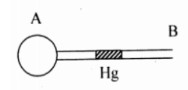
\includegraphics[width=0.2\linewidth]{figs/VN12-Y24-PH-SYL-011P-2}
	\end{center}

	\choice
	{\True $\SI{106}{\centi\meter^3}$}
	{$\SI{210}{\centi\meter^3}$}
	{$\SI{134}{\centi\meter^3}$}
	{$\SI{250}{\centi\meter^3}$}
	\loigiai{\begin{center}
			\begin{tabular}{C{4cm} C{3cm} C{4cm}}
				\colorbox{yellow}{\textcolor{red}{\textbf{Trạng thái 1}}} & $\xrightarrow[]{p_1=p_2}$ & \colorbox{yellow}{\textcolor{red}{\textbf{Trạng thái 2}}}\\
				$V_1=V+\SI{3}{\centi\meter^3}$ & &$V_2=V+\SI{5}{\centi\meter^3}$\\
				$T_1=\SI{273}{\kelvin}$ & & $T_2=\SI{278}{\kelvin}$
			\end{tabular}
		\end{center}
		$$\dfrac{V_1}{T_1}=\dfrac{V_2}{T_2}\Rightarrow V\approx\SI{106}{\centi\meter^3}.$$
	}
\end{ex}
\Closesolutionfile{ans}
\subsection{TRẮC NGHIỆM ĐÚNG/SAI}
\setcounter{ex}{0}
% ===================================================================
\begin{ex}
\immini{	Hiện nay, nồi áp suất là một trong các thiệt bị gia dụng được sử dùng phổ biến. Nồi áp suất giúp rút ngắn thời gian đun nấu, đa dạng chế độ nấu và an toàn cao nhờ hệ thống khoá nắp nồi khi chưa xả hết khí ra ngoài.
	\begin{enumerate}[label=\alph*)]
		\item Trong quá trình đun, áp suất bên trong nồi cao hơn áp suất khí quyển.
		\item Quá trình đun nấu diễn ra nhanh hơn do nước trong nồi áp suất sôi ở nhiệt độ thấp hơn $\SI{100}{\celsius}$.
		\item Van xả khí giúp cho khí và hơi nước trong nồi được xả ra ngoài một cách từ từ đến khi cân bằng với áp suất bên ngoài.
		\item Nếu không có khoá an toàn và mở nắp nồi khi khí chưa được xả ra ngoài thì nước trong nồi sẽ nhanh chóng chuyển thành hơi đồng thời phun ra ngoài.
	\end{enumerate}}
{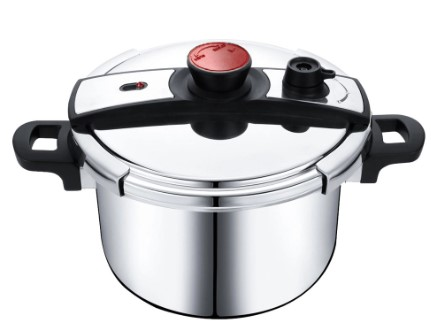
\includegraphics[scale=0.4]{figs/VN12-Y24-PH-SYL-011P-5}
}
	\loigiai{\begin{enumerate}[label=\alph*)]
			\item Đúng.
			\item Sai.
			\item Đúng.
			\item Đúng.
		\end{enumerate}
	}
\end{ex}
\subsection{BÀI TẬP TỰ LUẬN}
\setcounter{ex}{0}
% ===================================================================
\begin{ex}
	Khi tăng nhiệt độ của một lượng khí xác định từ $\SI{32}{\celsius}$ lên $\SI{117}{\celsius}$ và giữ áp suất không đổi thì thể tích khí tăng thêm $\SI{1.7}{\liter}$. Thể tích của lượng khí sau khi tăng nhiệt độ là bao nhiêu?
	\loigiai{\begin{center}
			\begin{tabular}{C{4cm} C{3cm} C{4cm}}
				\colorbox{yellow}{\textcolor{red}{\textbf{Trạng thái 1}}} & $\xrightarrow[]{p_1=p_2}$ & \colorbox{yellow}{\textcolor{red}{\textbf{Trạng thái 2}}}\\
				$V_1=V_2-\SI{1.7}{\liter}$ & &$V_2=?$\\
				$T_1=\SI{305}{\kelvin}$ & & $T_2=\SI{390}{\kelvin}$
			\end{tabular}
		\end{center}
		$$\dfrac{V_1}{T_1}=\dfrac{V_2}{T_2}\Rightarrow V_2=\SI{7.8}{\liter}.$$}
\end{ex}
% ===================================================================
\begin{ex}
	Khối lượng riêng không khí trong phòng ở nhiệt độ $\SI{27}{\celsius}$ lớn hơn khối lượng riêng của không khí ngoài sân nắng ở nhiệt độ $\SI{42}{\celsius}$ bao nhiêu lần. Biết áp suất không khí trong và ngoài phòng là như nhau.
	\loigiai{$$\dfrac{D_1}{D_2}=\dfrac{V_2}{V_1}=\dfrac{T_2}{T_1}=1,05.$$
	}
\end{ex}
% ===================================================================
\begin{ex}
	Khí ở lò thoát ra theo ống khói hình trụ. Ở đầu dưới, khí có nhiệt độ $\SI{727}{\celsius}$ và chuyển động với tốc độ $\SI{5}{\meter/\second}$. Áp suất khí coi như không đổi. Ở đầu trên của ống, khí có nhiệt độ $\SI{227}{\celsius}$. Tốc độ của khí ở đầu trên bằng bao nhiêu?
	\loigiai{\begin{center}
			\begin{tabular}{C{4cm} C{3cm} C{4cm}}
				\colorbox{yellow}{\textcolor{red}{\textbf{Trạng thái 1}}} & $\xrightarrow[]{p_1=p_2}$ & \colorbox{yellow}{\textcolor{red}{\textbf{Trạng thái 2}}}\\
				$V_1=v_1tS$ & &$V_2=v_2tS$\\
				$T_1=\SI{1000}{\kelvin}$ & & $T_2=\SI{500}{\kelvin}$
			\end{tabular}
		\end{center}
		$$\dfrac{V_1}{T_1}=\dfrac{V_2}{T_2}\Rightarrow v_2=\SI{2.5}{\meter/\second}.$$}
\end{ex}
	
	
